\problemname{Bell Ringing}

\emph{Method ringing} is used to ring bells in churches, particularly in England. Suppose there are
$6$ bells that have $6$ different pitches.
We assign the number $1$ to the bell highest in pitch, $2$ to the second highest, and so on.
When the $6$ bells are rung in some order---each of them exactly once---it is called a \emph{row}.
For example, $1, 2, 3, 4, 5, 6$ and $6, 3, 2, 4, 1, 5$ are two different rows.

An \emph{ideal} performance contains all possible rows, each played exactly once.
Unfortunately, the laws of physics place a limitation on any two consecutive rows;
when a bell is rung, it has considerable inertia and the ringer has
only a limited ability to accelerate or retard its cycle.
Therefore, the position of each bell can change by at most one between two consecutive rows.

In Figure~\ref{fig:bob}, you can see the pattern of a non-ideal performance, where
bells only change position by at most one.

\begin{figure}[h]
    \begin{center}
    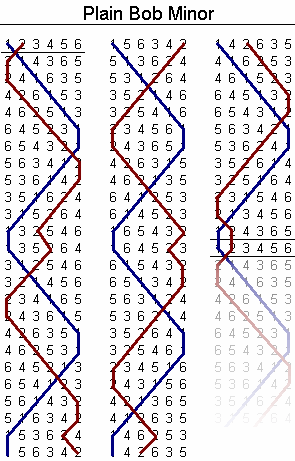
\includegraphics[height=0.65\textwidth]{Plain-bob-minor}
    \caption{A non-ideal performance respecting the inertia of bells. The trajectory of bell number
    $1$ is marked with a blue line and trajectory of bell number $2$ marked with a brown line.}
    \end{center}
    \label{fig:bob}
\end{figure}

Given $n$, the number of bells, output an ideal performance. All possible rows must be present
exactly once, and the first row should be $1, 2, \dots, n$.


\section*{Input}

The first and only line of input contains an integer $n$ such that $1 \leq n \leq 8$.

\section*{Output}

Output an ideal sequence of rows, each on a separate line. The first line should contain the row $1, 2,
\dots, n$ and each two consecutive lines should be at most $1$ step away from each other. Each row
should occur exactly once in the output.
